\chapter{Komponentenschnitt}
\begin{figure}[H]
    \centering
    \fbox{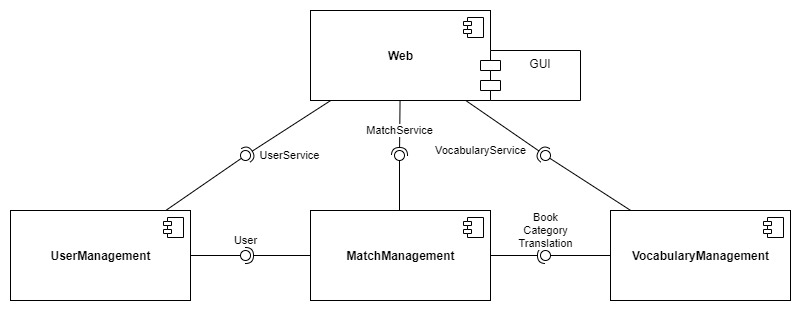
\includegraphics[width=0.99\textwidth-2\fboxsep-2\fboxrule]{Includes/Komponentendiagramm.jpg}}
    \caption{Komponentendiagramm}
    \label{komp}
\end{figure}
Wie in Abbildung \ref{komp} zu sehen ist, besteht die Software aus vier Komponenten. Im folgenden werden die Aufgaben dieser Komponenten näher beschrieben.
\section*{Web}
Die "Web" Komponente stellt die eigentliche Serveranwendung dar. Diese verwaltet somit den Zugriff über den Client bzw. der GUI auf die Anwendungslogik. Dementsprechend ist sie über Interfaces mit den anderen Komponenten verbunden.
\section*{UserManagement}
Diese Komponente ist für die Benutzerverwaltung zuständig. Dabei müssen Benutzer angelegt werden und sich amelden können. Neben der Verbindung zur "Web" Komponente ist auch eine Verbindung über die Klasse "User" zur "MatchManagement" Komponente notwendig, damit diese ihre Aufgaben erfüllen kann.
\section*{MatchManagement}
Die Komponente "MatchManagement" stellt die eigentliche Match- bzw. Spiele- oder auch Anwendungslogik zur Verfügung. Damit diese umfassend funktionieren kann benötigt sie die Klassen "Book", "Category" und "Translation" der "VocabularyManagement" Komponente. Zudem muss die "UserManagement" Komponente die Klasse "User" zu Verfügung stellen.
\section*{VocabularyManagement}
Zur Verwaltung der Vokabeldaten wird die "VocabularyManagement" Komponente herangezogen. Diese stellt der "MatchManagement" Komponente notwendige Klassen. Zudem erlaubt sie dem Benutzer über die "Web" Komponente neue Daten als Datei hochzuladen.
\clearpage
%- - - - - - - - - - - - - - - - - - - - - - - - - - - - - - - - - - - - - - - - - - - - - - - - - - - - - - -
\chapter{Schnittstellenbeschreibung}
Im Folgenden werden die Schnittstellen zwischen den Anwendungskomponenten und der "Web" Komponente beschrieben.
\section*{UserService}
Als Schnittstelle zwischen "Web" Komponente und "UserManagement" Komponente dient das "UserService" Interfaces. Dieses biete folgende Funktionalitäten:
\begin{lstlisting}
package vocab.services;

import vocab.domain.User;
import vocab.exceptions.ResourceNotFoundException;    
import java.sql.SQLException;

/**
 * The following interface provides methods to manage users.
 * @version 0.1
 */    
public interface UserService {
    /**
     * This method adds an new user.
     * @param username The name of the new user.
     * @param password The required password of the new user.
     * @return The method returns a the added user.
     * @throws SQLException The method throws a SQLException in case of the requested username is already in use.
     */
    User addUser(String username, String password) throws SQLException;

    /**
     * This method is for respective logging a user in.
     * @param username The name of the user.
     * @param password The required password of the user.
     * @return The method returns a User instance.
     * @throws ResourceNotFoundException The method throws an exception in case of the requested user could not be found.
     */
    User getUser(String username, String password) throws ResourceNotFoundException;

    /**
     * This method is used to get a user.
     * @param id The method requires the id representing the user.
     * @return The method return the requested user.
     * @throws ResourceNotFoundException The method throws an exception in case of the requested user could not be found.
     */
    User getUserById(Long id) throws ResourceNotFoundException;
}
\end{lstlisting}
\section*{MatchService}
Die Schnittstelle zwischen "Web" Komponente und der "MatchManagement" Komponente wird durch das "MatchService" Interfaces definiert. Dieses stellt folgende Funktionalitäten zur Verfügung:
\begin{lstlisting}
package vocab.services;

import vocab.domain.*;
import vocab.exceptions.ResourceNotFoundException;
import javax.persistence.OptimisticLockException;
import java.util.List;

/**
 * This interface provides methods to manage matches.
 * @version 0.1
 */
public interface MatchService {
    /**
     * This method can be used to create a new match.
     * @param user The method requires the user who creates the match.
     * @param book The method requires a book, used to play.
     * @return The method returns a new Match instance.
     */
    Match createMatch(User user, Book book);

    /**
     * This method can be used to access a match.
     * @param match_id The method requires the match_id representing the match.
     * @return The method returns a Match instance, or null in case of not finding a match with the match_id.
     * @throws ResourceNotFoundException The method throws an exception case of the match cannot be found.
     */
    Match getMatch(Long match_id) throws ResourceNotFoundException;

    /**
     * This method can be used to update a match persistent.
     * @param match The method requires the match to be updated.
     * @return The method returns a boolean representing the success of the method.
     * @throws OptimisticLockException The method throws an exception case of the match was already updated.
     */
    void updateMatch(Match match) throws OptimisticLockException;

    /**
     * This method can be used to get all matches with only one user.
     * @return The method returns a List of matches representing all matches with only one user.
     */
    List<Match> getAvailableMatches(User user);

    /**
     * This method is used to add a second user to a match.
     * @param user The user that should be added.
     * @param match_id The id ot the match.
     * @return The method returns the match that the second user was added.
     * @throws OptimisticLockException The method throws an exception case of the match was updated.
     */
    Match joinMatch(User user, Long match_id) throws OptimisticLockException, ResourceNotFoundException;

    /**
     * This method provides the functionality to answer a question.
     * @param answer The method requires a String instance representing the answer.
     * @param question The method requires the question instance that should be answered.
     * @param user The method requires the user that answers the question.
     * @return The method returns a boolean representing correctness of the give answer.
     */
    Boolean submitAnswer(String answer, Question question, User user);

    /**
     * This method provides the functionality to flag a match as finished.
     * @param match_id The method requires the id of the match that should be finished.
     * @throws ResourceNotFoundException The method throws an exception case of the match cannot be found.
     */
    void finishMatch(Long match_id) throws ResourceNotFoundException, OptimisticLockException;

    /**
     * This method provides the functionality to get a question.
     * @param question_id The method requires the id of the question.
     * @return The method returns the question, or null in case of not finding the question.
     * @throws ResourceNotFoundException The method throws an exception case of the question cannot be found.
     * @throws OptimisticLockException The method throws an exception case of the match was updated.
     */
    Question getQuestion(Long question_id) throws ResourceNotFoundException;

    /**
     * This method provides the functionality to start a round.
     * @param category The method requires the category that should be used in the round.
     * @param match The method requires the match that contains the round.
     * @return The method returns the round.
     * @throws OptimisticLockException The method throws an exception case of the match was updated.
     * @throws ResourceNotFoundException The method throws an exception case of the match cannot be found.
     */
    Round startRound(Category category, Match match) throws OptimisticLockException, ResourceNotFoundException;
}
\end{lstlisting}
\clearpage
\section*{VocabularyService}
Zwischen "Web" und der "VocabularyManagement" Komponente wird die Schnittstelle durch das "VocabularyService" Interfaces definiert. Dieses verfügt über folgende Funktionalitäten:
\begin{lstlisting}
package vocab.services;

import org.springframework.web.multipart.MultipartFile;
import vocab.domain.Book;
import vocab.domain.Category;
import vocab.exceptions.BadInputFileException;
import vocab.exceptions.ItemNotFoundException;
import java.io.File;
import java.util.List;

/**
 * This interface is can be used to manage the vocabulary.
 * @version 0.1
 */
public interface VocabularyService {
    /**
     * This method provides the access to all books written in a gameDirection.
     * @return The method returns a List instance of Books representing all playable Books.
     */
    List<Book> getBooks();

    /**
     * This method can be used to insert a file into the database.
     * @param file The method requires the file that should be inserted.
     * @return The method returns a boolean which indicates that te database was changed.
     * @throws BadInputFileException The method throws a exception if the provided file is not using the standard vocabulary format.
     */
    Boolean addFile(File file) throws BadInputFileException;

    /**
     * This method is used to get a category.
     * @param id The method requires the id representing the category.
     * @return The method returns the category, or null in case of not finding the requested category.
     * @throws ItemNotFoundException The method throws an exception in case there is no book with a matching id.
     */
    Category getCategory(Long id) throws ItemNotFoundException;

    /**
     * This method is used to get a book.
     * @param id The method requires the id representing the book.
     * @return The method returns the book, or null in case of not finding the requested book.
     * @throws ItemNotFoundException The method throws an exception in case there is no book with a matching id.
     */
    Book getBook(Long id) throws ItemNotFoundException;

    /**
     * This method is used to insert a multipart file into the database.
     * @param file The method requires the multipart file that should be inserted.
     * @return The method returns a boolean which indicates that te database was changed.
     * @throws BadInputFileException The method throws a exception if the provided file is not using the standard vocabulary format.
     */
    Boolean addMultipartFileHelper(MultipartFile file) throws BadInputFileException;
}    
\end{lstlisting}
\clearpage
%- - - - - - - - - - - - - - - - - - - - - - - - - - - - - - - - - - - - - - - - - - - - - - - - - - - - - - -
\chapter{Konzeptionelles Datenmodell}
\clearpage
%- - - - - - - - - - - - - - - - - - - - - - - - - - - - - - - - - - - - - - - - - - - - - - - - - - - - - - -
\chapter{Präsentationsschicht}
\clearpage
%- - - - - - - - - - - - - - - - - - - - - - - - - - - - - - - - - - - - - - - - - - - - - - - - - - - - - - -
\chapter{Frameworks}
\begin{itemize}
    \item Spring Boot
    \item JPA Hibernate
    \item Axios
    \item React
\end{itemize}
%- - - - - - - - - - - - - - - - - - - - - - - - - - - - - - - - - - - - - - - - - - - - - - - - - - - - - - -
\chapter{Ablaufumgebung}
\begin{table}[H]
    \begin{tabular}{p{0.32\textwidth}|p{0.66\textwidth}}
        Umgebung & Version \\
        \hline
        \hline
        Betriebssystem & Windows 10 \\
        Java & JDK 11 \\
        Maven & 4.0.0 \\
    \end{tabular}
\end{table}
\clearpage
%- - - - - - - - - - - - - - - - - - - - - - - - - - - - - - - - - - - - - - - - - - - - - - - - - - - - - - -